\chapter{Dimensionering}

Figur \ref{fig:hej} viser de nye byggefelter inden for henholdsvis delområde A og delområde B til Strøybergs Palæ (\citep{lokalplan}, s. 16). Denne rapport fokuserer på byggefeltet inden for delområde B, hvor ny bebyggelse, ifølge lokalplan 1-1-107, må opføres i 3 etager samt en tagetage og med en kælder maksimalt 2 m over terræn. Ved opførsel af ny bebyggelse i delområde B, skal to nuværende mindre bygninger fjernes. 

\begin{figure}[htbp]
	\centering
	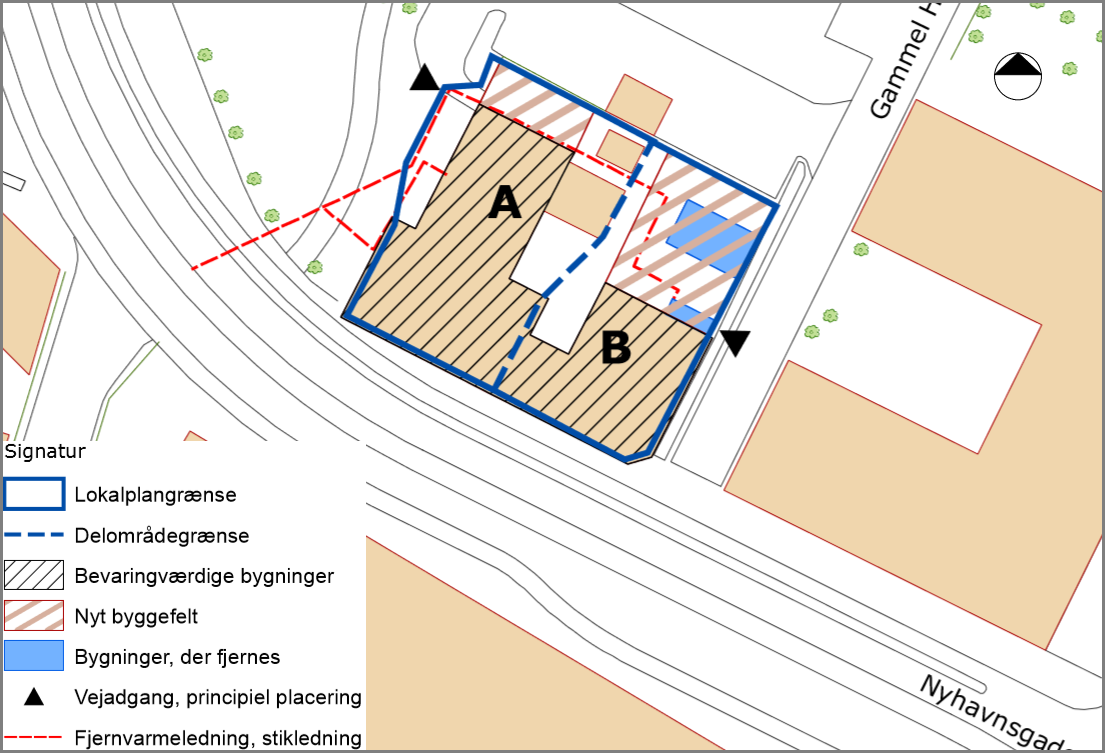
\includegraphics[width=0.8\textwidth]{billeder/signatur.png}
	\caption{Lokalplan 1-1-107, delområde A og B \citep{lokalplan[ bilag 2, s. 35]}}
	\label{fig:hej}
\end{figure}

Med udgangspunkt i lokalplan 1-1-107 har bygningen fået de størrelser og dimensioner, som ses på Figur \ref{fig:farvel}.
\newline \indent{     }  Tilbygningen bliver $12,\!5$ meter lang og 12 meter bred i henhold til den eksisterende bygningsbredde. Kælderen har en højde på i alt $3,\!25$ m, hvor $1,\!25$ m ligger over terræn. Stueetagen, 1. sal og 2. sal har hver især en højde på $4,\!9$ m og tagetagen har en højde på 3 meter med en hældning på $26,\!6$ grader. I alt er tilbygningen 19 m høj over terræn.

\begin{figure}[htbp]
	\centering
	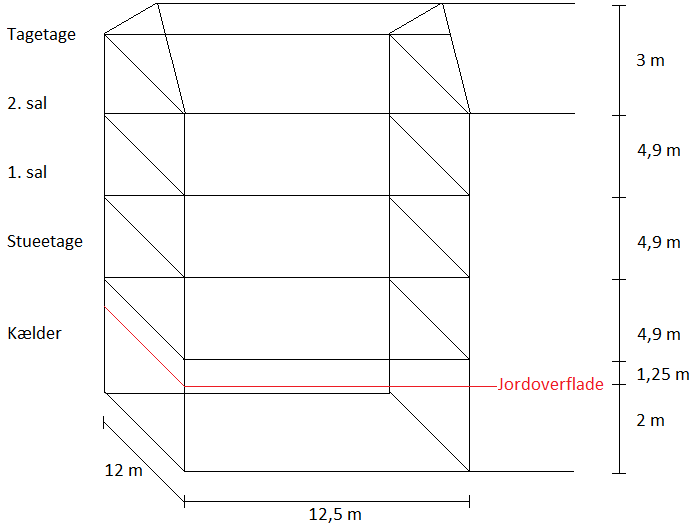
\includegraphics[width=0.7\textwidth]{billeder/tilbygning2.png}
	\caption{Tilbygningens dimensioner}
	\label{fig:farvel}
\end{figure}

For at kunne beregne de laster som påvirker tilbygningen, er der opstillet nedenstående statisk system for bygningen. Systemet er opstillet som en bjælkekonstruktion.
\newline
\newline
Beregningerne opdeles for to gavle og to facader. Det antages at gavlene hver er 12 m lang og 16 m høj, eksklusiv en gavltrekant med en højde på 3 m, og har 9 vinduer med dimensionerne; $0,\!95$ m bred og $1,\!5$ m høj.
\newline
\newline
De to facader er $12,\!5$ m lang og 16 m høj. Den har 11 vinduer, med samme mål som for vinduerne på gavlene, og en dør, som er $1,\!5$ m bred og $2,\!1$ m høj.
\newline
\newline
For at kunne beregne de laster, som påvirker tilbygningen, er der opstillet et statisk system for tilbygningen. Systemet er opstillet som en bjælkekonstruktion og indeholder tre rammekonstruktioner som vist på Figur \ref{fig:system}.

\begin{figure}[htbp]
	\centering
	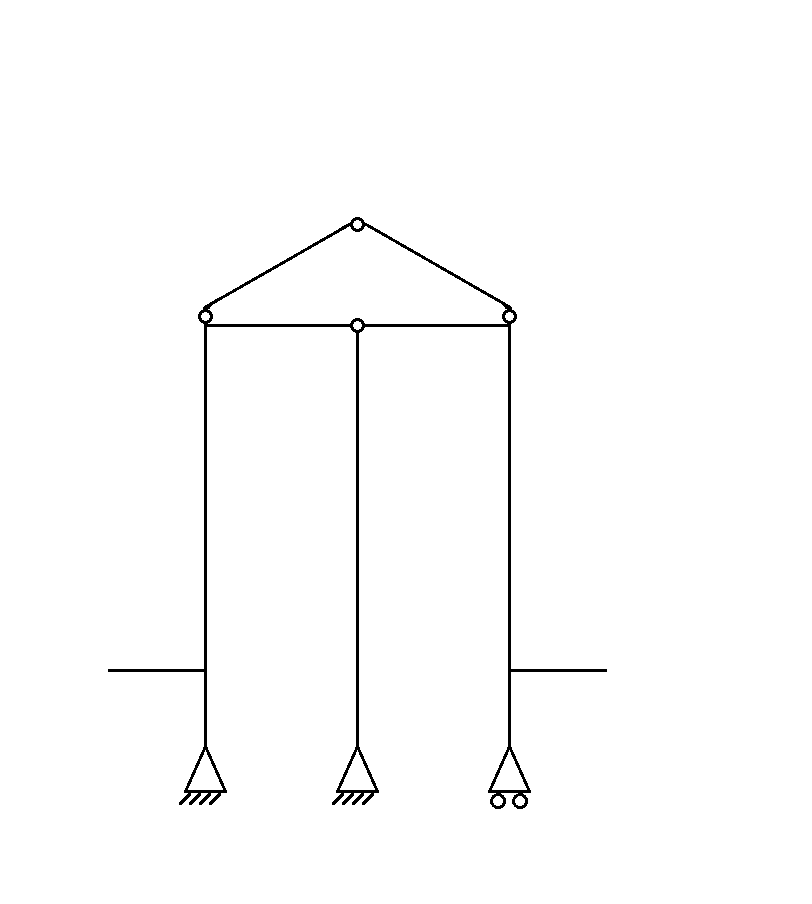
\includegraphics[width=0.3\textwidth]{billeder/del1statiskesystem.png}
	\caption{Statiske system}
	\label{fig:system}
\end{figure}

På disse rammekonstruktioner vil etagedækkene virke som en belastning, i stedet for at virke som en del af konstruktion. Dette er muligt, da der kan opsættes en samling mellem etagedækkene og stålkonstruktion, som ses på Figur \ref{fig:etage}.

\begin{figure}[htbp]
	\centering
	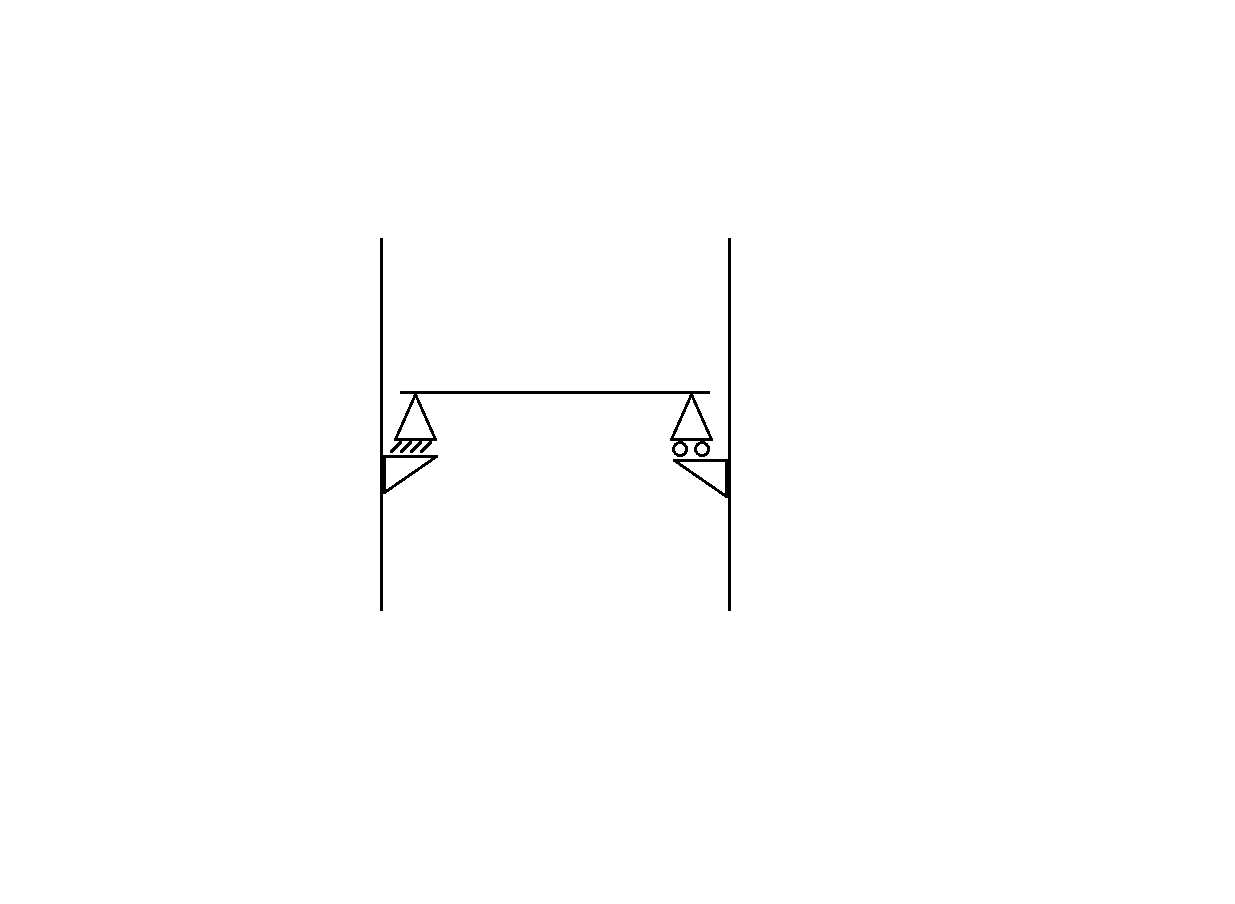
\includegraphics[width=0.2\textwidth]{billeder/etageovergang.png}
	\caption{Etageovergang på tilbygningen}
	\label{fig:etage}
\end{figure}

Med denne opstilling kan reaktionerne beregnes og der ud fra finde belastningen, som vil komme på funderingen, men først skal lasterne beregnes.

\section{Laster}
Tilbygningen til Strøybergs Palæ vil blive udsat for en række forskellige laster, både permanente- og variable laster, hvilke vil blive beregnet i dette afsnit således, at der senere hen kan opstilles lastkombinationer, regnes reaktionskræfter, snitkræfter, spændinger samt brudgrænse- og anvendelsesgrænsetilstande.

\subsection{Permanent last}
Egenlaster er permanente laster. For tilbygningen til Strøybergs Palæ beregnes disse laster gennem de gjorte antagelser samt de givne mål, som er illustreret på Figur \ref{fig:farvel}.
\newline
\newline
\textbf{Last fra væg}
\newline
\newline
\underline{Facade}
\newline
Facaderne antages for at være ens samt indeholde lige mange vinduer og døre. Der antages at være 11 vinduer og én dør pr. facade, hvilket illustreres på Figur \ref{fig:facade}.

\begin{figure}[htbp]
	\centering
	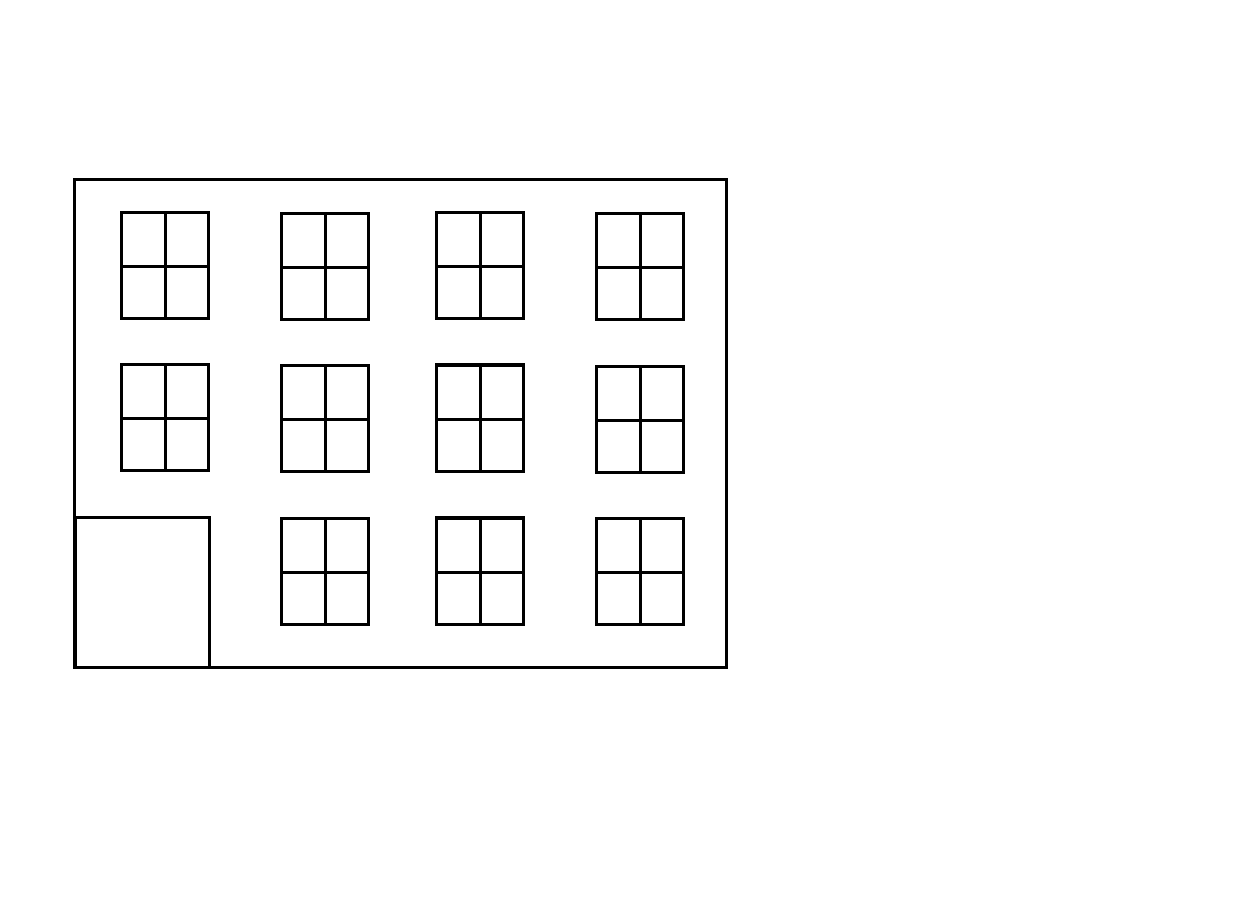
\includegraphics[width=0.8\textwidth]{billeder/facadenord.png}
	\caption{Facaden på øst- og vestsiden}
	\label{fig:facade}
\end{figure}
 
\indent{     }  Ét vindue regnes til være $0,\!95$ m bred og $1,\!5$ m høj TJEK MED MICHAEL! + KILDE. Døren antages at være $1,\!5$ m bred og $2,\!1$ m høj KILDE. Arealet for én facade bestemmes til:
\begin{center}
	$12,\!5 m\cdot 16,\!0 m - (1,\!5 m\cdot0,\!95 m\cdot11 + 1,\!5 m\cdot 2,\!1 m)=181,\!175 m^2$
\end{center}

Til beregning af væggens egenlast vides det, at der skal påregnes en indervæg og et isoleringslag, mens den ydervæggen ikke er en del af det statiske system og dermed ikke skal medregnes.
\newline \indent{     }  Ifølge KILDE(http://www.bolius.dk/tunge-indvendige-vaegge-19288) aflæses en typisk indervæg til at være 130 mm tyk, og det antages, at denne værdi benyttes til tilbygningen af Strøybergs Palæ. Dermed kan værdien for indervæggen af facaden nu bestemmes ved at gange facadens areal uden viduer og dør med tykkelsen, hvorefter denne værdi ganges med densiteten for mursten, hvilket er $1500,\!0 \frac{kg}{m^3}$:
\begin{center}
	$181,\!175 m^2\cdot 130 mm\cdot 1500,\!0 \frac{kg}{m^3}\cdot 9,\!82 \frac{m}{s^2}=35329,\!125 kg$
\end{center}

Denne værdi omregnes til $N$ ved at gange med tyngdeaccelerationen:
\begin{center}
	$35329,\!125 kg\cdot 9,\!82 \frac{m}{s^2}=346,\!932 kN$
\end{center}

I og med facaderne er identiske ganges de $346,\!932 kN$ med 2:
\begin{center}
	$346,\!932 kN\cdot 2=693,\!864 kN$
\end{center}

Isoleringslaget skal ifølge KILDE$(http://www.byggeriogenergi.dk/media/5932/indv_efterisolering_massive_murede_vaegge_ok.pdf)$ være 100 mm tyk. Det antages, at typen af isolering har densiteten $30 \frac{kg}{m^3}$ KILDE (http://www.rockwool.dk/produkter/u/7429/bygningsisolering/bd-60-flexibatts).
\newline \indent{     }  Facadens areal uden vinduer og dør med tykkelsen, hvorefter denne værdi ganges med densiteten for isoleringen:
\begin{center}
	$181,\!175 m^2\cdot 0,1 \cdot 30 \frac{kg}{m^3}\cdot 9,\!82 \frac{m}{s^2}=5,\!337 kN$
\end{center}

I og med facaderne er identiske ganges de $5,\!337 kN$ med 2:
\begin{center}
	$5,\!337 kN\cdot 2=10,\!675 kN$
\end{center}

\underline{Gavl}
\newline
Da den ene gavl ligger op ad den nuværende bygning, vil der ikke være vinduer på denne gavl, mens der antages at være 9 vinduer, identiske med dem for facaden, for gavlen, der ikke ligger op ad den nuværende bygning, som kan ses på Figur \ref{fig:gavl}.

\begin{figure}[htbp]
	\centering
	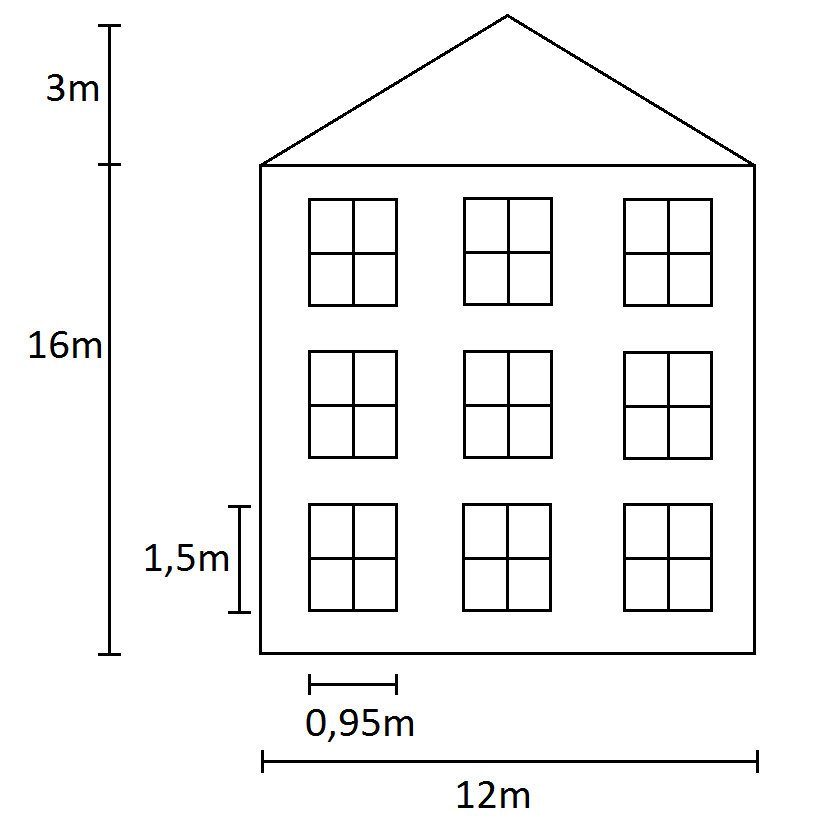
\includegraphics[width=0.6\textwidth]{billeder/facadevestellerost.png}
	\caption{Dimensioner for tagetagen}
	\label{fig:gavl}
\end{figure}

Til forskel for facadens areal, har gavlene også arealet for tagetagen, som har dimensionerne der ses på Figur \ref{fig:tagetage}. Arealet for facaden der ikke ligger op ad den nuværende bygning bestemmes dermed til:
\begin{center}
	$12 m\cdot 16 m + 3 m\cdot 12 m \cdot 0,\!5 - 1,\!5 m\cdot 0,\!95 m \cdot 9=197,\!175 m^2$
\end{center}

\begin{figure}[htbp]
	\centering
	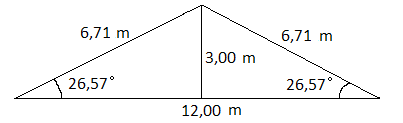
\includegraphics[width=0.7\textwidth]{billeder/Tagmedvinkel.png}
	\caption{Dimensioner for tagetagen}
	\label{fig:tagetage}
\end{figure}

Ligesom for facaderne skal der også påregnes en indervæg og et isoleringslag for gavlene, og det antages at værdierne for facaderne er ens med gavlene med hensyn til tykkelse og densitet for indervæg og isolering.
\newline
\newline
Værdien for indervæggen bestemmes til:
\begin{center}
	$197,\!175 m^2\cdot 130 mm\cdot 1500,\!0 \frac{kg}{m^3}\cdot 9,\!82 \frac{m}{s^2}=377,\!570 kN$
\end{center}

Værdien for isolering bestemmes til:
\begin{center}
	$197,\!175 m^2\cdot 100 mm\cdot 30 \frac{kg}{m^3}\cdot 9,\!82 \frac{m}{s^2}=5,\!809 kN$
\end{center}

Hermed regnes værdierne nu for gavlen, der ligger op ad den nuværende bygning. 
\newline \indent{     }  Arealet af gavlen bestemmes til:
\begin{center}
	$12 m\cdot 16 m + 3 m\cdot 12 m \cdot 0,\!5=210,\!0 m^2$
\end{center}

Værdien for indervæggen bestemmes til:
\begin{center}
	$210,\!0 m^2\cdot 130 mm\cdot 1500,\!0 \frac{kg}{m^3}\cdot 9,\!82 \frac{m}{s^2}=402,\!129 kN$
\end{center}

Værdien for isolering bestemmes til:
\begin{center}
	$210,\!0 m^2\cdot 100 mm\cdot 30 \frac{kg}{m^3}\cdot 9,\!82 \frac{m}{s^2}=6,\!187 kN$
\end{center}

\textbf{Last fra gulv}
\newline
Det antages at bygnings etager kun består af gulv, dvs. ingen skillevægge, trapper og andre former for genstande, der mindsker mængden af gulv. Derfor er den samlede mængde gulv pr. etage $12,\!5 m\cdot 12,\!0 m=150,\!0 m^2$.
\newline \indent{     }  Fire ud af de fem etager består af bærende gulv, hvor den sidste, kælderetagen, ligger på fundamentet. Et bærende gulv antages at bestå af et armeret betondæk nederst, der oftest er mellem 80 mm og 200 mm tyk. Der antages, at den er 120 mm tyk, hvorpå der ligger bjælker. Bjælkernes opgave er at lede og overføre lasterne ud i understøtning. Derefter vil ligge et undergulv, mellemgulv og til sidst selve gulvbelægningen, og mellem betondækket og undergulvet lægges isoleringen. 
\newline \indent{     }  Først bestemmes gulvets last for en etage, hvorefter denne ganges denne med fire, da der er fire etager foruden kælderetagen. Betondækkets andel beregnes først, da både længden, bredden og tykkelsen kendes. 
\newline
\newline
Rumfanget af betonen for én etage bestemmes til:
\begin{center}
	$12,\!5 m\cdot 12,\!0 m\cdot 120 mm=18,\!0 m^3$
\end{center}

Rumfanget ganges med betons densitet, som er $2400 \frac{kg}{m^3}$, KILDE (http://materials.dk/links/D5x5\%20Betons\%20densitet.pdf), hvorefter denne værdi ganges med tyngdeaccelerationen, for at få værdien i $kN$, som der ganges med 4 for at få lasten for alle fire etager:
\begin{center}
	$18,\!0 m^3\cdot 2400 \frac{kg}{m^3}\cdot 9,82 \frac{m}{s^2}\cdot 4=1693,440 kN$
\end{center}

Der er behov for bjælker, som hver er $6,\!25$ m lang, da de er halvdelen af tilbygningens længde, $140,\!0$ mm høj og $140,\!0$ mm bred KILDE $(http://www.danskbyggeri.dk/files/Filbibliotek/Erhvervs-\%20og\%20byggeteknik/Tolerancer/52615.toemrer_net.pdf)$. Disse anlægges langs med tilbygningen. For at bestemme hvor mange bjælker, der er behov for, divideres længden af tilbygningen med 400 mm, da der skal være 400 mm imellem hver bjælke KILDE.
\begin{center}
	$\frac{12,\!5 m}{400 mm}=31,\!25$ bjælker
\end{center} 

Da der ikke kan optræde $31,\!25$ bjælker rundes der op til 32 bjælker.
\newline
\newline
Rumfanget af én bjælke, som består af to bjælker med længden $6,\!25$ m, ganges med bjælkens densitet fir tørrumvægt af træ KILDE (http://trae.dk/index.asp?page=\%2FDokumenter\%2FDokument.asp\%3FDokumentID\%3D124), hvorefter denne værdi ganges med tyngdeaccelerationen og ganges med 4: 
\begin{center}
	$7,\!840 m^3\cdot 510 \frac{kg}{m^3}\cdot 9,\!82 \frac{m}{s^2}\cdot 4=157,\!057 kN$
\end{center}

Isoleringsarealet for tilbygningen er det samlede gulvareal minus det areal, som bjælkerne ligger på:
\begin{center}
	$150,\! m^2 - (140 mm\cdot 12,\!5 m\cdot 32)=94,\!0 m^2$
\end{center}

Isoleringslaget har samme højde som bjælkerne og har en densitet på $30 \frac{kg}{m^3}$ KILDE (http://www.rockwool.dk/produkter/u/7429/bygningsisolering/bd-60-flexibatts). Dermed kan værdien for isolering bestemmes til:
\begin{center}
	$94,\!0 m^2\cdot 140 mm\cdot 30 \frac{kg}{m^3}\cdot 9,\!82 \frac{m}{s^2}\cdot 4=15,\!508 kN$
\end{center}

Gulvbelægningen antages for at være linoleumsgulv med en højde på $2,\!5 mm$ KILDE! med en densitet på $2,\!9 \frac{kg}{m^3}$ KILDE (http://www.kjeldtoft.com/upl/website/download-brochurer-/DesktopTekniskespecifikationer.pdf). Dermed kan værdien for linoleumsgulv bestemmes til:
\begin{center}
	$2,\!5 mm\cdot 12,\!5 m\cdot 12,\!0 m\cdot 2,\!9 \frac{kg}{m^3}\cdot 9,\!82 \frac{m}{s^2}\cdot 4=0,\!043 kN$
\end{center}

\textbf{Last fra tag}
\newline
Det antages at taget, som benyttes, er et mellemtungt tag, som har værdien $600 \frac{N}{m^2}$, (http://www.ringstedspaer.dk/konstruktioner.htm) og det er et sadeltag med teglsten. Der er derfor fundet en middelværdi for lasten fra taget til systemet. 
\newline
\newline
Tagets areal bestemmes ud fra Figur \ref{fig:tagetage}:
\begin{center}
	$6,\!7 m\cdot 12,\!5 m \cdot 2=167,\!500 m^2$
\end{center}

Arealet ganges med værdien for mellemtungt tag:
\begin{center}
	$167,\!500 m^2\cdot 600 \frac{N}{m^2}=100,\!500 kN$
\end{center}

\subsection{Variable laster}
Af variable laster optræder der både snelast, vindlast og nyttelast på bygningen, og disse udregnes efter Dansk Standard Eurocode 1991.

\subsubsection{Snelast}
Til at beregne hvordan snelasten påvirker tilbygningen anvendes den karaktiske snelast og formlen:
\begin{center}
$s=\mu_iC_eC_ts_k$
\end{center}
\begin{itemize}
	\item[-] $s$: karakteristisk snelast
	\item[-] $\mu_i$: formfaktoren for snelasten, som sættes til 0.8 \citep[ tabel 5.2 kapitel 5.3]{EU91}
	\item[-] $C_e$: eksponeringsfaktoren
	\item[-] $C_t$: termisk faktor, som sættes til $1,\!0$ \citep[ kapitel 5.2]{EU91}
	\item[-] $s_k$: karakteristisk terrænværdi, som sættes til $1 \frac{kN}{m^2}$ \citep[ kapitel 4.1]{EU91}
\end{itemize}
Til at bestemme den karakteristiske snelast, beregnes eksponeringsfaktoren $C_e$.
\newline
\newline
Eksponeringsfaktoren, $C_e$, bestemmes ved:
\begin{center}
$C_e=C_{top}C_s$
\end{center}
\begin{itemize}
	\item[-] $C_{top}$: topografi faktor, som sættes til $1,\!0$ \citep[ tabel 5.1 kapitel 5.2]{EU91}
	\item[-] $C_s$: størrelse faktor, som sættes til $1,\!0$ \citep[ kapitel 5.2]{EU91}
\end{itemize}
Eksponeringsfaktoren kan nu bestemmes til:
\begin{center}
$C_e=1,\!0\cdot 1,\!0=1,\!0$
\end{center}
Strøybergs Palæ har et saddeltag, og dermed skal der tages højde for fire lasttilfælde, som ses på Figur \ref{fig:sne}. Derudover ganges snetilfældets værdi med 6,25 m, som er halvdelen af tilbygningens længde, hvilket gøres, da det statiske system er opdelt i tre rammer, for at få værdien ud i $\frac{kN}{m}$.

\begin{figure}[htbp]
	\centering
	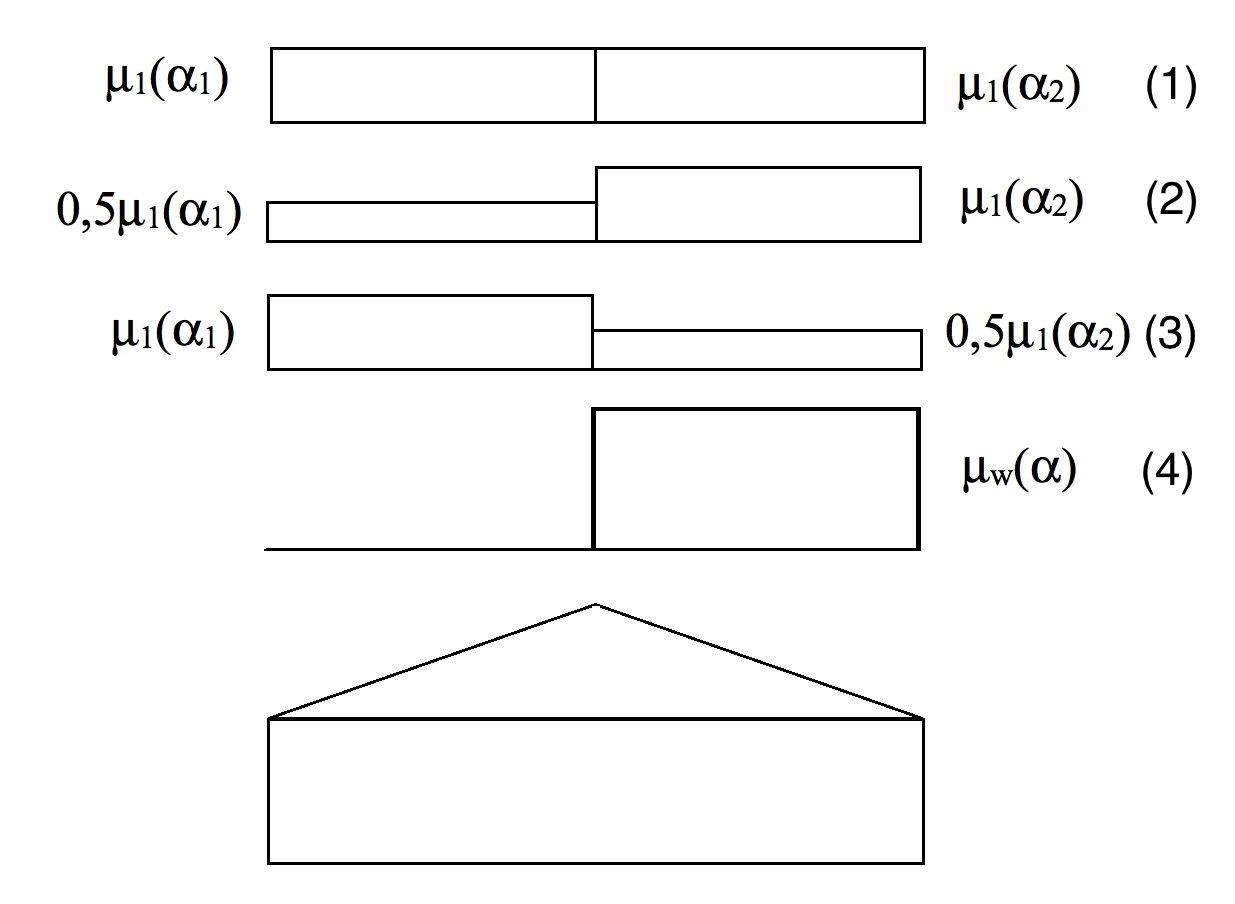
\includegraphics[width=0.6\textwidth]{billeder/snelasttilfaelde.png}
	\caption{Fordeling af sne i de fire tilfælde}
	\label{fig:sne}
\end{figure}

\underline{Snetilfælde 1}
\begin{center}
$s_1=0,\!8\cdot 1.0\cdot 1,\!0\cdot 1 \frac{kN}{m^2}\cdot 6,\!25 m=5,\!0 \frac{kN}{m}$
\end{center}
\underline{Snetilfælde 2 og 3}
\begin{center}
$s_2=\frac{1}{2}\cdot 0,\!8\cdot 1,\!0\cdot 1,\!0\cdot 1 \frac{kN}{m^2}\cdot 6,\!25 m=2,\!5 \frac{kN}{m}$
\end{center}
\underline{Snetilfælde 4}
\begin{center}
	$s_4=\mu_wC_eC_ts_k \frac{kN}{m^2}$
\end{center}
\begin{itemize}
	\item[-] $\mu_w$: formfaktoren, som sættes til $1,\!2$ eftersom $\alpha$ er $26,\!565^{\circ}$ \citep[ kapitel 5.3.3]{EU91}
\end{itemize}
Den karakteristiske snelast for lasttilfælde 4 kan nu bestemmes til:
\begin{center}
	$s_4=1,\!2\cdot 1,\!0\cdot 1,\!0\cdot 1 \frac{kN}{m^2}6,\!25 m=7,\!5 \frac{kN}{m}$
\end{center}
I og med at lasttilfælde 4 giver den største last, anvendes denne til videre beregning.

\subsubsection{Vindlast}
For vindlasten skal der regnes en nettovindlast, som er forskellige mellem den udvendige og den indvendige last. Lasterne skal ud i $\frac{kN}{m}$, som skal anvendes til lastkombinationer.
\newline \indent{     }  For Strøybergs Palæ regnes der en nettovindlast for siden af bygningen og for taget af bygningen. Dette gøres for tre vindretninger, nord, øst og vest, da sydsiden af tilbygningen kommer i forlængelse af en anden bygning, og derfor formodes denne vindlast ikke at have særlig stor betydning for tilbygningen.
\newline
\newline
Til at bestemme vindlasten på tilbygningens vindtryk på de udvendige flader anvendes følgende formel:	
\begin{center} 
	$w_e=q_p(z_e)c_{pe}$
\end{center}
\begin{itemize}
	\item[-] $q_p$: peakhastighedstrykket
	\item[-] $z_e$: referencehøjden for det udvendige vindtryk, som sættes til 19 m for taget og 16 m for tilbygningen uden tag \ref{fig:tagetage}
	\item[-] $c_{pe}$: formfaktoren for det udvendige vindtryk
\end{itemize}

Til at bestemme vindlasten på tilbygningens vindtryk på de indvendige flader anvendes følgende formel:
\begin{center} 
	$w_i=q_p(z_i)c_{pi}$
\end{center}
\begin{itemize}
	\item[-] $q_p$: peakhastighedstrykket
	\item[-] $z_i$: referencehøjden for det indvendige vindtryk, som sættes lig $z_e$ \citep[ kapitel 7.2.9]{EU91}
	\item[-] $c_{pi}$: formfaktoren for det indvendige vindtryk
\end{itemize}

Nedenfor gives et beregningseksempel for beregning af $q_p$ på tilbygningens udvendige side med højden 19 m. Beregningerne for udvendig med højden 16 m og indvendig for både 19 m og 16 m kan ses i bilag, hvor fremgangsmåden er ens som den viste blot med andre værdier fra de samme tabeller som anvendes i eksemplet. INDSÆTTE REFERENCE HER!
\newline
\newline
Den maksimale belastning fra vinden, peakhastighedstrykket $q_p$, bestemmes ved:
\begin{center}
$q_p(z_e)=[1+7I_v(z_e)]\frac{1}{2}pv_m^2(z_e)$
\end{center}
\begin{itemize}
	\item[-] $I_v$: vindturbulens
	\item[-] $\rho$: densiteten for luft $1,\!25 \frac{kg}{m^3}$ KILDE
	\item[-] $v_m$: middelvindhastigheden
\end{itemize}
For at bestemme peakhastigheden, beregnes først vindturbulens $I_v(z)$ samt middelvindhastigheden $v_m$.
\newline
\newline
Vindturbulens, $I_v(z)$, bestemmes ved:
\begin{center}
$I_v(z)=\frac{\sigma_v}{V_m(z)}=\frac{k_1}{c_0(z)\cdot ln(\frac{z}{z_0})}$
\end{center}
\begin{itemize}
	\item[-] $k_1$: turbulensfaktor, sættes til $1,\!0$ \citep[ kapitel 4.4]{EU91}
	\item[-] $c_0(z)$: orografifaktoren, som sættes til $1,\!0$ \citep[ kapitel 4.3.1]{EU91}
	\item[-] $z$: højde, som er 19 m
	\item[-] $z_0$: ruhedslængde, som sættes til $1,\!0$ for terrænkategori IV \citep[ tabel 4.1 kapitel 4.3.2]{EU91}
\end{itemize}
Vindturbulensen kan nu bestemmes til:
\begin{center}
$I_v(z)=\frac{1,\!0}{1,\!0\cdot ln(\frac{19}{1,\!0})}=0,\!340$
\end{center}
Middelvindhastigheden, $v_m$, bestemmes ved:
\begin{center}
$v_m(z)=c_r(z)c_0(z)v_b$
\end{center}
\begin{itemize}
	\item[-] $c_r(z)$: ruhedsfaktor
	\item[-] $v_b$: basisvindhastigheden
\end{itemize}
Til at bestemme middelvindhastigheden, beregnes basisvindhastigheden samt ruhedsfaktor.
\newline
\newline
Basisvindhastigheden, $v_b$, bestemmes ved:
\begin{center}
$v_b=c_{dir}c_{season}v_{b,0}$
\end{center}
\begin{itemize}
	\item[-] $c_{dir}$: retningsfaktor, som sættes til $1,\!0$ \citep[ tabel 1a kapitel 4.2]{EU91}
	\item[-] $c_{season}$: årstidsfaktor, som sættes til $1,\!0$ \citep[ tabel 1b kapitel 4.2]{EU91}
	\item[-] $v_{b,0}$: grundværdi for basisvindhastigheden, som sættes til 24 $\frac{m}{s}$, da dette er gældende for størstedelen af Danmark \citep[ kapitel 4.2]{EU91}
\end{itemize}
Basisvindhastigheden kan nu bestemmes til:
\begin{center}
$v_b=1,\!0\cdot 1,\!0\cdot 24 \frac{m}{s}=24 \frac{m}{s}$
\end{center}
Ruhedsfaktor, $c_r(z)$, bestemmes ved:
\begin{center}
$c_r(z)=k_rln(\frac{z}{z_0})$
\end{center}
\begin{itemize}
	\item[-] $k_r$: terrænfaktor
\end{itemize}
Terrænfaktoren, $k_r$, bestemmes ved:
\begin{center}
$k_r=0,\!19\cdot (\frac{z_0}{z_{0,II}})^{0,\!07}$
\end{center}
\begin{itemize}
	\item[-] $z_{0,II}$: værdi for ruhedslængde for terrænkategori II, som sættes til $0,\!05$ \citep[ kapitel 4.3.2]{EU91}
\end{itemize}
\begin{center}
$k_r=0.19\cdot (\frac{1,\!0}{z_{0,\!05}})^{0,\!07}=0,\!234$
\end{center}
Ruhedsfaktor kan nu bestemmes til:
\begin{center}
$c_r(z)=0,\!234\cdot ln(\frac{19}{1.0})=0,\!690$
\end{center}
Middelvindhastigheden kan nu bestemmes til:
\begin{center}
$v_m(z)=0,\!690\cdot 1,\!0\cdot 24 \frac{m}{s}=16,\!569 \frac{m}{s}$
\end{center}
Peakhastighedstrykket $q_p$ i højden z, kan nu bestemmes til:
\begin{center}
$q_p(z_e)=[1+7\cdot 0,\!340]\cdot \frac{1}{2}\cdot 1,\!25 \frac{kg}{m^3}\cdot (16,\!569 \frac{m}{s})^2=0,\!579 \frac{kN}{m^2}$
\end{center}

HVAD GØR VI NU??

\begin{figure}[htbp]
	\centering
	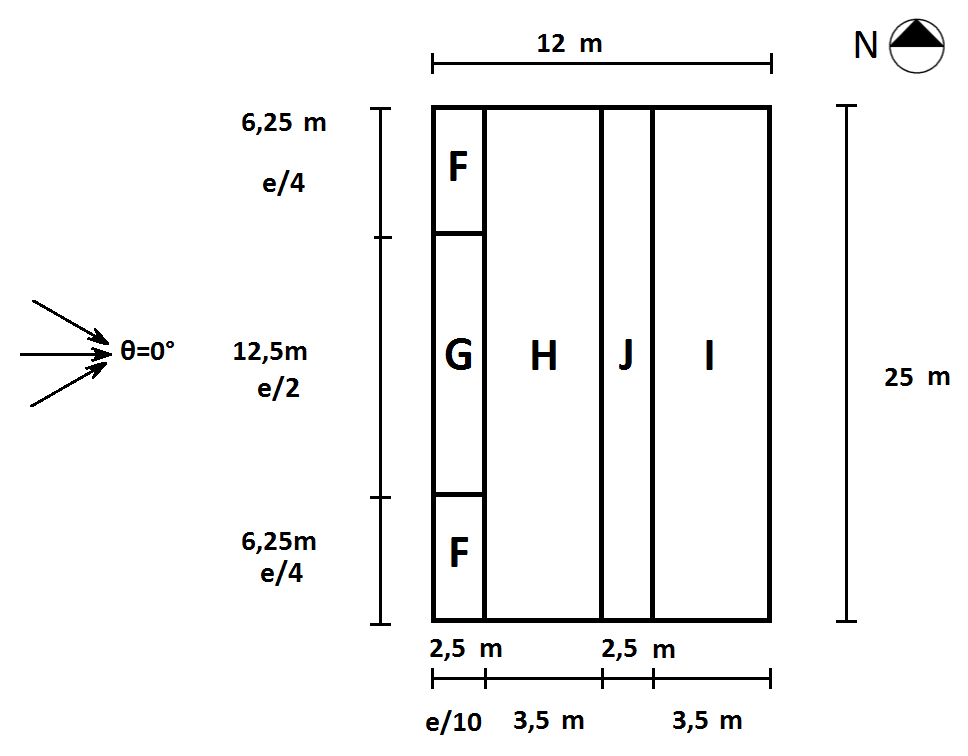
\includegraphics[width=0.5\textwidth]{billeder/opdeling.png}
	\caption{Zoneinddeling af taget}
	\label{fig:tag}
\end{figure}

For alle zoner bestemmes $c_{pe,10}$. Der opstilles en lineær ligning med sammenhæng mellem $c_{pe,10}$ værdierne og graderne 15 og 30. Herefter indsættes taghældningen, $26,\!565^{\circ}$ i ligningen og værdien for $c_{pe,10}$ i den pågældende zone fås.
\newline
\newline
\underline{Zone F}
\newline
Ud fra \citep[ tabel 7.4a kapitel 7.2.5]{EU91} er de negative værdier for zone F: $-0,\!9$ og $-0,\!5$. Her ud fra fås ligningen, og $c_{pe,10,neg}$ bestemmes:
\begin{center}
	$f(\alpha)=0,\!0267\cdot \alpha - 1,\!3 \to c_{pe,10,neg}=-0,\!592$
\end{center}
De positive værdier for zone F er: $0,\!2$ og $0,\!7$. Her ud fra fås ligningen, og $c_{pe,10,pos}$ bestemmes:
\begin{center}
	$f(\alpha)=0,\!0333\alpha - 0,\!3 \to c_{pe,10,pos}=0,\!585$
\end{center}

\underline{Zone G}
\newline
De negative værdier for zone G er: $-0,\!8$ og $-0,\!5$. Her ud fra fås ligningen, og $c_{pe,10,neg}$ bestemmes:
\begin{center}
	$f(\alpha)=0.02\alpha - 1,\!1 \to c_{pe,10,neg}=-0,\!569$
\end{center}
De positive værdier for zone G er: $0,\!2$ og $0,\!7$. Her ud fra fås ligningen, og $c_{pe,10,pos}$ bestemmes:
\begin{center}
	$f(\alpha)=0.0333\alpha - 0,\!3 \to c_{pe,10,pos}=0,\!585$
\end{center}

\underline{Zone H}
\newline
De negative værdier for zone H er: $-0,\!3$ og $-0,\!2$. Her ud fra fås ligningen, og $c_{pe,10,neg}$ bestemmes:
\begin{center}
	$f(\alpha)=0.00667\alpha - 0\!4 \to c_{pe,10,neg}=-0.223$
\end{center}
De positive værdier for zone H er: $0,\!2$ og $0,\!4$. Her ud fra fås ligningen, og $c_{pe,10,pos}$ bestemmes:
\begin{center}
	$f(\alpha)=0,\!0133\alpha - 1,\!178\cdot 10^{-16} \to c_{pe,10,pos}=0,\!354$
\end{center}

\underline{Zone I}
\newline
Den negative værdi for zone I er: $-0,\!4$. Her ud fra fås ligningen, og $c_{pe,10,neg}$ bestemmes:
\begin{center}
	$f(\alpha)=-5,\!234\cdot 10^{-18}\alpha - 0,\!4 \to c_{pe,10,neg}=-0,\!4$
\end{center}
Den positive værdi for zone I er: $0,\!0$. Her ud fra fås ligningen, og $c_{pe,10,pos}$ bestemmes:
\begin{center}
	$f(\alpha)=0,\!0 \to c_{pe,10,pos}=0,\!0$
\end{center}

\underline{Zone J}
\newline
De negative værdier for zone J er: $-1,\!0$ og $-0,\!5$. Her ud fra fås ligningen, og $c_{pe,10,neg}$ bestemmes:
\begin{center}
	$f(\alpha)=0,\!0333\alpha - 1,\!5 \to c_{pe,10,neg}=-0,\!615$
\end{center}
Den positive værdi for zone J er: $0,\!0$. Her ud fra fås ligningen, og $c_{pe,10,pos}$ bestemmes:
\begin{center}
	$f(\alpha)=0.0 \to c_{pe,10,pos}=0.0$
\end{center}
INDSÆTTE DET SIDSTE!

\subsection{Nyttelast}
Ud fra \citep[ tabel 6.2 kapitel 6.3.1.2]{EU91} aflæses den jævnt fordelte last, $q_k$, for kategori A1, som er bolig og lokale adgangsveje, til at være $1,\!5 \frac{kN}{m^2}$. Denne last beregnes for alle etager på tilbygningen samlet set.
\begin{center}
	$Q_{K3}=q_k A etageantal$
\end{center}
\begin{itemize}
	\item[-] A: arealet af én etage, som sættes til $150,\!0 m^2$
	\item[-] antal etager for tilbygningen er 5, men der ses bort fra kælderetagen
\end{itemize}
Nyttelasten kan nu bestemmes til:
\begin{center}
	$Q_{K3}=1,\!5 \frac{kN}{m^2}\cdot 150,\!0 m^2\cdot 4=900,\!0 kN$
\end{center}

\section{Lastkombinationer}
INTROTEKST
\newline
\newline
\underline{Lastkombination 1: Egenlast}
\newline
Den regningsmæssige egenlasten bestemmes ud fra følgende formel:
\begin{center}
	$E_{d,1}=\gamma_{G1}K_{FI}G_{K1}$
\end{center}
\begin{itemize}
	\item[-] $\gamma_{G1}$: partialkoefficienten for den permanente last, som sættes til $1,\!2$ \citep[ tabel A 1.2(B+C) anneks A.1.3.1]{EU90}
	\item[-] $K_{FI}$: konsekvensklasse CC3, som sættes til $1,\!1$ \citep[ tabel A 1.2(A) anneks A.1.3.1]{EU90}
	\item[-] $G_{K1}$: karakteristisk egenlast for den permanente last [kN], som sættes til $3437,\!86$ kN
\end{itemize}
Den regningsmæssige egenlast kan nu bestemmes til:
\begin{center}
	$E_{d,1}=1,\!2\cdot 1,1\cdot 3437,\!86 kN=4,\!538\cdot 10^3 kN$
\end{center}
\underline{Lastkombination 2: Vindlast dominerende}
\newline
Den regningsmæssige last, for vindlast dominerende, bestemmes ud fra følgende formel:
\begin{center}
	$E_{d,2}=\gamma_{G1}K_{FI}G_{K1}+\gamma_{Q1}K_{FI}Q_{K1}+\gamma_{Q2}\Psi_{0,2}K_{FI} Q_{K2}+\gamma_{Q3}\Psi_{0,3}K_{FI}Q_{K3}$
\end{center}
\begin{itemize}
	\item[-] $\gamma_{Q1}$: partialkoefficienten, som sættes til 1,5 \citep[ tabel A 1.2(B+C) anneks A.1.3.1]{EU90}
	\item[-] $Q_{K1}$: karakteristisk nyttelast for vind, som sættes til X
	\item[-] $\gamma_{Q2}$: partialkoefficenten, som sættes til 1,5 \citep[ tabel A 1.2(B+C) anneks A.1.3.1]{EU90}
	\item[-] $\Psi_{0,2}$: $\Psi$-faktor, som sættes til 0,0, ved vindlast dominerende \citep[ tabel A 1.1 anneks A.1.2.2]{EU90}
	\item[-] $Q_{K2}$: karakteristisk nyttelast for sne, som sættes til Y
	\item[-] $\gamma_{Q3}$: partialkoefficenten, som sættes til $1,\!5$ \citep[ tabel A 1.2(B+C) anneks A.1.3.1]{EU90}
	\item[-] $\Psi_{0,3}$: $\Psi$-faktor, som sættes til 0,5 \citep[ tabel A 1.1 anneks A.1.2.2]{EU90}
	\item[-] $Q_{K3}$: karakteristisk nyttelast for bolig, som sættes til $900,\!0$ kN
\end{itemize}
Den regningsmæssige værdi for vindlast dominerende kan nu bestemmes til:
\begin{center}
	$E_{d,2}=$
\end{center}

\underline{Lastkombination 3: Snelast dominerende}
\newline
Den regningsmæssige last, for snelast dominerende, bestemmes ud fra følgende formel:
\begin{center}
 	$E_{d,3}=\gamma_{G1}K_{FI} G_{K1}+\gamma_{Q1}\Psi_{0,\!1}K_{FI}Q_{K1}+\gamma_{Q2}K_{FI}Q_{K2}+\gamma_{Q3}\Psi_{0,3}K_{FI}Q_{K3}$
\end{center}
\begin{itemize}
	\item[-] $\Psi_{0,\!1}$: $\Psi$-faktor, som sættes til $0,\!3$ \citep[ tabel A 1.1 anneks A.1.2.2]{EU90}
\end{itemize}
Den regningsmæssige værdi for snelast dominerende kan nu bestemmes til:
\begin{center}
	$E_{d,3}=$
\end{center}

\underline{Lastkombination 4: Nyttelast dominerende}
\newline
Den regningsmæssige last, for nyttelast dominerende, bestemmes ud fra følgende formel:
\begin{center}
	$E_{d,4}=\gamma_{G1}K_{FI}G_{K1}+\gamma_{Q1}\Psi_{0,\!1}K_{FI}Q_{K1}+\gamma_{Q2}\Psi_{0,\!2}K_{FI}Q_{K2}+\gamma_{Q3}K_{FI}Q_{K3}$
\end{center}
\begin{itemize}
	\item[-] $\Psi_{0,\!2}$: $\Psi$-faktor, som sættes til $0,\!3$ \citep[ tabel A 1.1 anneks A.1.2.2]{EU90}
\end{itemize}
Den regningsmæssige værdi for nyttelast dominerende kan nu bestemmes til:
\begin{center}
	$E_{d,4}=$
\end{center}